\subsection{Равномерно распределенные матрицы поворота}

Следующий алгоритм к получению равномерно распределенных матриц поворота состоит из двух шагов:
\begin{enumerate}
\item равномерно распределенный поворот вокруг оси $OZ$
\item поворот, приводящий к равномерному на сфере положению северного полюса
\end{enumerate} 

Первый шаг осуществить легко; пусть случайная величина $x_1$ равномерно распределена на отрезке $[0, 1]$, тогда матрица $R$ осуществляет равномерно распределенный поворот вокруг оси $OZ$ 
\begin{gather}
R =
\begin{bmatrix}
\cos \lb 2 \pi x_1 \rb & \sin \lb 2 \pi x_1 \rb & 0 \\
- \sin \lb 2 \pi x_1 \rb & \cos \lb 2 \pi x_1 \rb & 0 \\
0 & 0 & 1
\end{bmatrix} \label{rmatrix} 
\end{gather}

Второй шаг может быть выполнен при помощи \textit{преобразования Хаусхолдера} (Householder transform). Точка $z = (0, 0, 1)$  может быть перенесена в любую точку сферу при помощи отражения относительно плоскости, перпендикулярной вектору $\bar{zp}$ и проходящей через центр координат $O$. Такое отражение описывается \textit{Хаусхолдеровской матрицей}
\begin{gather}
		H = 1 - 2 v v^\top, \notag
\end{gather}
где $v$ -- единичный вектор, параллельный $\bar{zp}$. Взяв комбинацию хаусхолдеровского отражения и инверсии мы получим поворот, т.к. детерминант такого преобразования будет равен $\det(\cdot) = + 1$ (матрица преобразования будет равна $-H$). Таким образом, искомоая матрица поворота равна
\begin{gather}
		M = - HR \notag
\end{gather}

Матрица поворота $M$ будет равномерно распределена внутри $SO(3)$, если $H$ равномерно преобразует Северный полюс в любую точку на сфере, а $R$ описывает равномерный поворот вокруг $OZ$. Оператор $H$ будет удовлевторять поставленному условию, если мы возьмем
\begin{gather}
		v = 
		\begin{bmatrix}
				\cos \lb 2 \pi x_2 \rb \sqrt{x_3} \\
				\sin \lb 2 \pi x_2 \rb \sqrt{x_3} \\
				\sqrt{1 - x_3}
		\end{bmatrix}, \notag
\end{gather}
где $x_2$, $x_3$ -- равномерно распределены на $[0, 1]$. В таком случае матрица $H$ принимает следующий вид
\begin{gather}
		H = 1 - 2 v v^\top = 
		\begin{bmatrix}
			1 - 2 \cos^2 \lb 2 \pi x_2 \rb x_3 & -2 \sin \lb 2 \pi x_2 \rb \cos \lb 2 \pi x_2 \rb x_3 & - 2 \cos \lb 2 \pi x_2 \rb \sqrt{x_3 \lb 1 - x_3 \rb} \\
			- 2 \sin \lb 2 \pi x_2 \rb \cos \lb 2 \pi x_2 \rb x_3 & 1 - 2 \sin^2 \lb 2 \pi x_2 \rb x_3 & -2 \sin \lb 2 \pi x_2 \rb \sqrt{x_3 \lb 1 - x__3 \rb} \\
		- 2 \cos \lb 2 \pi x_2 \rb \sqrt{x_3 \lb 1 - x_3 \rb} & - 2 \sin \lb 2 \pi x_2 \rb \sqrt{x_3 \lb 1 - x_3 \rb} & 2 x_3 - 1
		\end{bmatrix} \notag
\end{gather}

Действие $H$ на вектор $z$ приводит к вектору $p$, компоненты которого равны
\begin{gather}
		 p = H z = \lb 1 - 2 v v^\top \rb \begin{bmatrix} 0 \\ 0 \\ 1 \end{bmatrix} =
		\begin{bmatrix}
				- 2 \cos \lb 2 \pi x_2 \rb \sqrt{x_3 \lb 1 - x_3 \rb} \\
				- 2 \sin \lb 2 \pi x_2 \rb \sqrt{x_3 \lb 1 - x_3 \rb} \\
				2 x_3 - 1
		\end{bmatrix} \notag
\end{gather}

Заметим, что если положить $\sin \phi = - 2 \sqrt{x_3 \lb 1 - x_3 \rb}$, то тогда $\cos \phi = 2 x_3 - 1$. Действительно,
\begin{gather}
	\sin^2 \phi + \cos^2 \phi = \left[ - 2 \sqrt{x_3 \lb 1 - x_3 \rb} \right]^2 + \left[ 2 x_3 - 1 \right]^2 = 1 \notag
\end{gather}

То есть, вектор $p$ может быть представлен в следующей форме
\begin{gather}
	p = 
	\begin{bmatrix}
		\cos \lb 2 \pi x_2 \rb \sin \varphi \\
		\sin \lb 2 \pi x_2 \rb \sin \varphi \\
		\cos \varphi
	\end{bmatrix} = 
	\begin{bmatrix}
		\cos \lb 2 \pi x_2 \rb \sqrt{z} \\
		\sin \lb 2 \pi x_2 \rb \sqrt{z} \\
		\sqrt{1 - z}
	\end{bmatrix}. \notag
\end{gather}
Следовательно $p$ равномерно распределен на сфере, т.к. азимутальный угол и косинус полярного угла $\cos \varphi = 2 x_3 - 1$ распределены равномерно на $[-1, 1]$. Для упрощения компонент вектора переобозначим $\sqrt{z} = \sqrt{x_3 \lb 1 - x_3 \rb}, \sqrt{1 - z} = 2 x_3 - 1 $. Итак, схема алгоритма представлена ниже.

\begin{algorithm}
\begin{algorithmic}[1]
\caption{Scheme of [3]} \label{randrot}
\State $x_1$, $x_2$, $x_3$ $\gets$ 3 random variables uniformly distributed over $[0, 1]$  
\State Pick a rotation about the pole: $\theta \gets 2 \pi x_1$  
\State Pick a direction to deflect the pole: $\phi \gets 2 \pi x_2$
\State Pick the amount of pole deflection: $z \gets x_3$.
\State Construct a vector to perform the reflection: 
v = 
\begin{bmatrix}
	\cos \phi \sqrt{z} \\
	\sin \phi \sqrt{z} \\
	\sqrt{1 - z}
\end{bmatrix}
\State Construct the rotation matrix by combining two simple rotations: first rotate about the $Z$-axis, then rotate the $Z$-axis to a random orientation: 
$
M \gets \lb 2 v v^\top - 1 \rb
\begin{bmatrix}
		\cos \theta & \sin \theta & 0 \\
		-\sin \theta & \cos \theta & 0 \\
		0 & 0 & 1
\end{bmatrix}
$.
\end{algorithmic}
\end{algorithm}

\begin{lstlisting}
#include <iostream>
#include <random>
#include <Eigen/Dense>

using namespace std;
using namespace Eigen;

//a Mersenne Twister pseudo−random generator of 32−bit numbers with a state size of 19937 bits 
random_device rd;
mt19937 eng( rd() );
uniform_real_distribution<double> distr( 0.0, 1.0);

void rotationMatrix( Matrix3d &m )
{
	double theta = 2 * M_PI * distr( eng ); // a rotation about the pole
	double phi = 2 * M_PI * distr( eng ); // a direction to deflect the pole 
	double z = distr( eng ); // the amount of pole deflection	 
	double sz = sqrt( z );

	// a vector to perform the reflection
	Vector3d v ( cos(phi) * sz, sin(phi) * sz, sqrt(1 - z) );
	// the Householder matrix
	Matrix3d s = 2 * v * v.transpose() - Matrix<double, 3, 3>::Identity();

	Matrix3d r;
   	r << cos(theta), sin(theta), 0,
		-sin(theta), cos(theta), 0,
		0, 0, 1;
	
	m = s * r;
}

int main( int argc, char* argv[] )
{
	int n = atoi( argv[1] );
	
	// initial vector
	Vector3d v ( 0.0, 0.0, 1.0 );
	// resulting vector
	Vector3d r;

	for ( int i = 0; i < n; i++ )
	{
		// filling rotation matrix
    	Matrix3d m;
    	rotationMatrix( m );

		// performing a random rotation of OZ-vector
		r = m * v;
		
		// displaying the components of resulting vector
		cout << r(0) << " " << r(1) << " " << r(2) << endl;
	}

    return 0;
}
\end{lstlisting}

Пример программы на C++ с применением библиотеки линейной алгебры $Eigen$. Программа принимает на вход количество рассчитываемых векторов $n$. Внутри главного цикла генерируется по описанному алгоритму случайная матрица поворота и применяется для поворота вектора $v = \left[ 0, 0, 1 \right]$. На выходе получаем $n$ равномерно распределенных на сфере векторов.

\begin{figure}[ht!]
		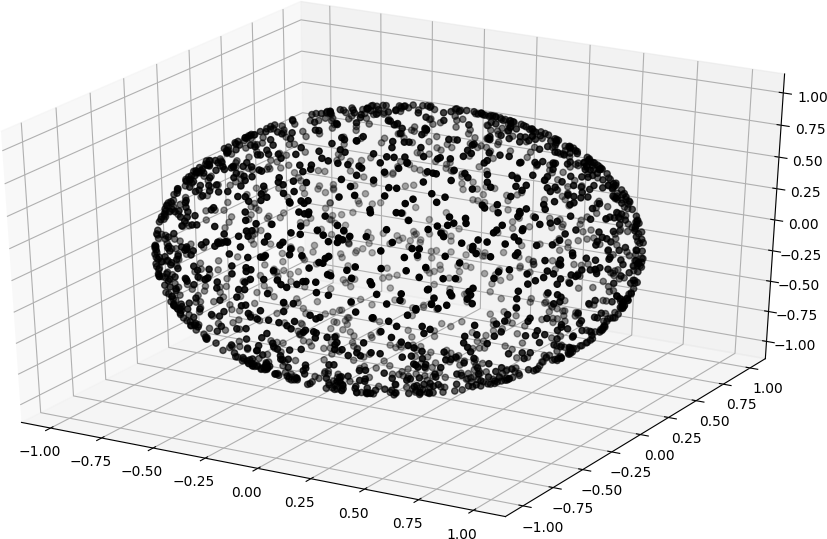
\includegraphics[width=\textwidth]{../pictures/sphere_dots.png}
		\caption{Пример равномерно распределенных на сфере точек, полученных в результате приведенной выше программы. 2000 точек.}
\end{figure}


